\chapter{GPU Libraries: cuBLAS, cuDNN, Thrust, and CUTLASS}\label{ch:libraries}
\sloppy

\begin{center}\small\textit{Do not rewrite what NVIDIA perfected --- learn to stand on 10\,000 engineer-hours of tuning.}\end{center}

\noindent\fbox{\parbox{\dimexpr\linewidth-2\fboxsep-2\fboxrule}{%
\textbf{From zero: no library expertise assumed.} We start from a familiar idea: a well-tuned library saves you from hand-writing every loop. On the CPU you call \texttt{BLAS} for matrices; on the GPU the same insight holds, but the library must also hide warps, tiling, Tensor Cores, and memory coalescing. First intuition, then APIs.}}
\vspace{0.4em}

\section*{Learning Outcomes}
After this chapter you will be able to:
\begin{enumerate}[label=(L\arabic*)]
    \item explain why GPU libraries outperform naive kernels and when to use them;
    \item call cuBLAS for \texttt{gemm} with correct handle, leading dimension, and transpose flags;
    \item describe cuDNN tensor descriptors and why convolution needs workspace;
    \item write Thrust code using device vectors and fused transforms;
    \item outline CUTLASS hierarchical tiling and how it exposes Tensor Core control.
\end{enumerate}

\section{Why Libraries Beat Hand-Written Kernels}
A naive $N\!\times\!N$ matrix multiply does $O(N^{3})$ work and $O(N^{2})$ data movement. The performance gap between a triple loop and a tuned library is $20$--$100\times$ because the library does: (i) tiling to fit shared memory, (ii) double-buffered async copies, (iii) warp-level matrix instructions, and (iv) auto-tuned tile sizes per architecture. Reimplementing all four is months of work; calling a library is one function.

Think of it as the GPU analogue of \texttt{sort()} vs.\ bubble sort: correctness is easy, near-peak efficiency is not. Libraries also track new hardware --- Hopper's \texttt{wgmma} appears first in CUTLASS, months before textbook kernels catch up.

\begin{definition}[GPU compute library]
A pre-compiled, auto-tuned collection of kernels plus a host API that abstracts tiling, data layout, and hardware intrinsics, exposing a stable interface (e.g., \texttt{cublasSgemm}) while internally selecting the fastest algorithm for the current GPU, data type, and shape.
\end{definition}

\begin{figure}[h]\centering
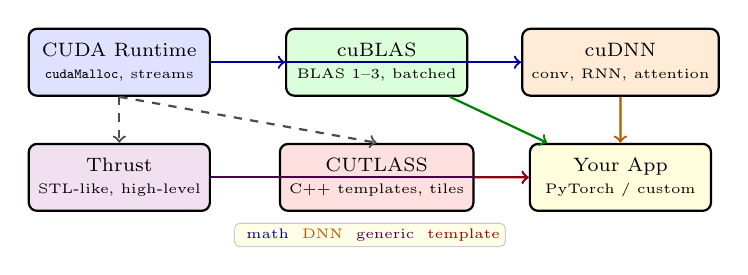
\begin{tikzpicture}[font=\scriptsize, scale=0.86,
  box/.style={draw, thick, rounded corners=3pt, minimum width=2.3cm, minimum height=0.85cm, align=center}]
  \node[box, fill=blue!12] (cuda) at (0,0) {CUDA Runtime\\{\tiny\texttt{cudaMalloc}, streams}};
  \node[box, fill=green!14] (cublas) at (3.8,0) {cuBLAS\\{\tiny BLAS 1--3, batched}};
  \node[box, fill=orange!16] (cudnn) at (7.4,0) {cuDNN\\{\tiny conv, RNN, attention}};
  \node[box, fill=violet!12] (thrust) at (0,-1.7) {Thrust\\{\tiny STL-like, high-level}};
  \node[box, fill=red!12] (cutlass) at (3.8,-1.7) {CUTLASS\\{\tiny C++ templates, tiles}};
  \node[box, fill=yellow!14] (app) at (7.4,-1.7) {Your App\\{\tiny PyTorch / custom}};
  \draw[->, thick, blue!60!black] (cuda) -- (cublas);
  \draw[->, thick, blue!60!black] (cuda) -- (cudnn);
  \draw[->, thick, green!50!black] (cublas) -- (app);
  \draw[->, thick, orange!70!black] (cudnn) -- (app);
  \draw[->, thick, violet!60!black] (thrust) -- (app);
  \draw[->, thick, red!60!black] (cutlass) -- (app);
  \draw[->, thick, gray!60!black, dashed] (cuda.south) -- (thrust.north);
  \draw[->, thick, gray!60!black, dashed] (cuda.south) -- (cutlass.north);
  \node[font=\tiny, fill=yellow!10, draw=gray!40, rounded corners=2pt, inner sep=2pt] at (3.7,-2.55) {\textcolor{blue!60!black}{$\blacksquare$ math} \textcolor{orange!70!black}{$\blacksquare$ DNN} \textcolor{violet!60!black}{$\blacksquare$ generic} \textcolor{red!60!black}{$\blacksquare$ template}};
\end{tikzpicture}
\caption{GPU library stack. All build on the CUDA runtime; domain libraries (cuBLAS/cuDNN) sit beside generic tools (Thrust/CUTLASS) and compose into applications.}
\label{fig:lib-stack}
\end{figure}

\section{cuBLAS: The Workhorse for Linear Algebra}
BLAS levels: L1 vector ops ($O(n)$), L2 matrix-vector ($O(n^{2})$), L3 matrix-matrix ($O(n^{3})$). GPU speedups grow with arithmetic intensity, so L3 \texttt{gemm} is where cuBLAS shines --- often $>90\%$ of peak.

Key API pattern: create a \texttt{cublasHandle\_t}, set stream with \texttt{cublasSetStream}, then call \texttt{cublasSgemm} / \texttt{cublasGemmEx}. Column-major is default (Fortran legacy); C row-major users transpose logically via \texttt{CUBLAS\_OP\_T} or set \texttt{CUBLAS\_LT} order. \texttt{lda, ldb, ldc} are leading dimensions, not $N$ --- stride between columns.

\begin{center}
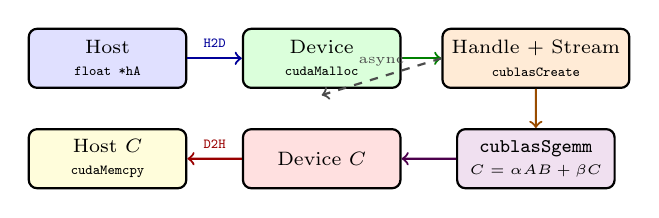
\begin{tikzpicture}[font=\scriptsize, scale=0.85,
  blk/.style={draw, thick, rounded corners=3pt, align=center, minimum width=2.0cm, minimum height=0.75cm}]
  \node[blk, fill=blue!12] (h) at (0,0) {Host\\{\tiny\texttt{float *hA}}};
  \node[blk, fill=green!14] (d) at (3.2,0) {Device\\{\tiny\texttt{cudaMalloc}}};
  \node[blk, fill=orange!16] (handle) at (6.4,0) {Handle + Stream\\{\tiny\texttt{cublasCreate}}};
  \node[blk, fill=violet!12] (gemm) at (6.4,-1.5) {\texttt{cublasSgemm}\\{\tiny $C=\alpha AB+\beta C$}};
  \node[blk, fill=red!12] (c) at (3.2,-1.5) {Device $C$};
  \node[blk, fill=yellow!14] (back) at (0,-1.5) {Host $C$\\{\tiny\texttt{cudaMemcpy}}};
  \draw[->, thick, blue!60!black] (h) -- (d) node[midway, above, font=\tiny] {\texttt{H2D}};
  \draw[->, thick, green!50!black] (d) -- (handle);
  \draw[->, thick, orange!60!black] (handle) -- (gemm);
  \draw[->, thick, violet!60!black] (gemm) -- (c);
  \draw[->, thick, red!60!black] (c) -- (back) node[midway, above, font=\tiny] {\texttt{D2H}};
  \draw[->, thick, gray!60!black, dashed] (handle.west) -- (3.2,-0.55) node[midway, above, font=\tiny] {async};
\end{tikzpicture}
\end{center}

Batched \texttt{gemm} matters for small matrices (e.g., attention heads): one call launches many tiny multiplies with one overhead. \texttt{cublasGemmStridedBatchedEx} adds mixed precision (\texttt{fp16} in, \texttt{fp32} accumulate) to use Tensor Cores automatically.

\begin{lstlisting}[language=C++, caption={cuBLAS SGEMM with handle, stream, and error check. Column-major $\alpha=1,\beta=0$.}]
#include <cublas_v2.h>
cublasHandle_t h; cublasCreate(&h);
cudaStream_t s; cudaStreamCreate(&s);
cublasSetStream(h, s);
int N=2048; float alpha=1,beta=0;
float *dA,*dB,*dC;
cudaMalloc(&dA,N*N*sizeof(float));
cudaMalloc(&dB,N*N*sizeof(float));
cudaMalloc(&dC,N*N*sizeof(float));
// ... fill dA,dB via cudaMemcpyAsync(..., s)
cublasSgemm(h, CUBLAS_OP_N, CUBLAS_OP_N, N,N,N,
            &alpha, dA,N, dB,N, &beta, dC,N);
cudaStreamSynchronize(s);
cublasDestroy(h);
\end{lstlisting}

Common pitfall: forgetting \texttt{cublasSetMathMode(h, CUBLAS\_TENSOR\_OP\_MATH)} --- without it, large gemms may not use Tensor Cores and run $4$--$8\times$ slower on Ampere+.

\section{cuDNN: Deep Learning Primitives}
cuDNN accelerates convolutions, RNNs, and fused attention. Unlike cuBLAS's flat arrays, cuDNN uses \emph{descriptors}: \texttt{cudnnTensorDescriptor\_t}, \texttt{cudnnFilterDescriptor\_t}, \texttt{cudnnConvolutionDescriptor\_t}. You describe shapes, strides, data type, and layout (\texttt{NCHW} vs.\ \texttt{NHWC}); cuDNN picks the fastest algorithm via \texttt{cudnnFindConvolutionForwardAlgorithm}.

Why the indirection? Convolution can lower to GEMM (\texttt{im2col} + gemm), use FFT, or use Winograd --- each wins on different shapes. cuDNN benchmarks candidates autotuning-style during \texttt{Find} and caches the choice. Workspace bytes trade memory for speed; \texttt{cudnnGetConvolutionForwardWorkspaceSize} tells you how much to allocate.

\begin{center}
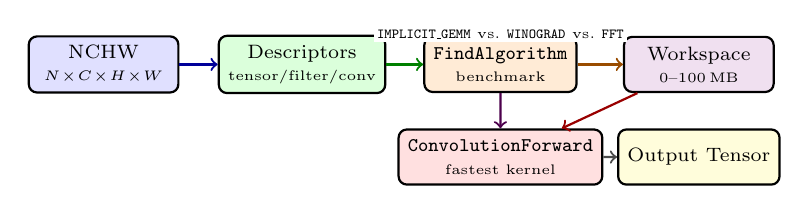
\begin{tikzpicture}[font=\scriptsize, scale=0.84,
  t/.style={draw, thick, rounded corners=3pt, minimum width=1.9cm, minimum height=0.70cm, align=center}]
  \node[t, fill=blue!12] (nchw) at (0,0) {NCHW\\{\tiny $N\!\times\!C\!\times\!H\!\times\!W$}};
  \node[t, fill=green!14] (desc) at (3.0,0) {Descriptors\\{\tiny tensor/filter/conv}};
  \node[t, fill=orange!16] (find) at (6.0,0) {\texttt{FindAlgorithm}\\{\tiny benchmark}};
  \node[t, fill=violet!12] (ws) at (9.0,0) {Workspace\\{\tiny 0--100\,MB}};
  \node[t, fill=red!12] (exec) at (6.0,-1.4) {\texttt{ConvolutionForward}\\{\tiny fastest kernel}};
  \node[t, fill=yellow!14] (out) at (9.0,-1.4) {Output Tensor};
  \draw[->, thick, blue!60!black] (nchw) -- (desc);
  \draw[->, thick, green!50!black] (desc) -- (find);
  \draw[->, thick, orange!60!black] (find) -- (ws);
  \draw[->, thick, violet!60!black] (find) -- (exec);
  \draw[->, thick, red!60!black] (ws) -- (exec);
  \draw[->, thick, gray!60!black] (exec) -- (out);
  \node[font=\tiny, fill=white, inner sep=1pt] at (6.0,0.45) {\texttt{IMPLICIT\_GEMM} vs.\ \texttt{WINOGRAD} vs.\ \texttt{FFT}};
\end{tikzpicture}
\end{center}

Fused ops (\texttt{cudnnConvolutionBiasActivationForward}) keep intermediates in registers/shared memory, cutting DRAM traffic --- the same fusion that drives Transformer speedups.

\section{Thrust and CUTLASS: Two Ends of Abstraction}
\emph{Thrust} is STL for GPUs: \texttt{thrust::device\_vector}, \texttt{transform}, \texttt{reduce}, \texttt{sort}. It picks backend (CUDA, TBB, OpenMP) at compile time. Productivity is high; control over tiling is low --- fine for preprocessing, not for squeezing the last $30\%$ of matmul.

\emph{CUTLASS} is the opposite: C++ templates where you compose \texttt{ThreadblockTile} $\to$ \texttt{WarpTile} $\to$ \texttt{InstructionTile}. You pick tile sizes, pipeline stages, epilogues, and the template elaborates to a kernel using \texttt{mma.sync} or Hopper \texttt{wgmma}. NVIDIA ships CUTLASS as the reference for new hardware features; PyTorch's fast kernels often are CUTLASS instantiations.

\begin{lstlisting}[language=C++, caption={Thrust: device vectors, transform, and reduce on the GPU.}]
#include <thrust/device_vector.h>
#include <thrust/transform.h>
#include <thrust/reduce.h>
thrust::device_vector<float> a(1<<20, 1.0f), b(1<<20, 2.0f), c(1<<20);
// c = a + b using a functor (lambda needs __host__ __device__)
thrust::transform(a.begin(), a.end(), b.begin(), c.begin(),
                  [] __host__ __device__ (float x, float y){ return x+y; });
float sum = thrust::reduce(c.begin(), c.end(), 0.0f, thrust::plus<float>());
// sum == 3 * 2^20 ; no explicit kernel, no cudaMalloc
\end{lstlisting}

Choosing: prototype with Thrust/cuBLAS, fuse with cuDNN, and when roofline says you are still compute-bound and need custom layouts, drop to CUTLASS. The three interoperate --- CUTLASS can consume cuBLASLt layouts, and Thrust can wrap raw device pointers via \texttt{thrust::device\_ptr}.

\begin{remark}
Library version lock is real: cuBLAS 12.x requires CUDA 12.x and driver $\ge$525. Pin versions in Docker, and prefer \texttt{cublasLt} / \texttt{cudnn} 8+ which decouple heuristics from the binary via JSON plan caches.
\end{remark}

\section{cuBLASLt, Mixed Precision, and Common Pitfalls}
\texttt{cublasLt} is the lightweight, more explicit cousin of cuBLAS. It exposes \emph{matmul descriptors}, \emph{algorithm heuristics}, and \emph{epilogues} (bias + ReLU) that fuse without extra passes. Instead of one \texttt{Sgemm} call, you build a \texttt{cublasLtMatmulDesc}, set compute type (\texttt{CUBLAS\_COMPUTE\_32F}), scale type, and let \texttt{cublasLtMatmulAlgoGetHeuristic} rank candidates for your exact $M,N,K$.

Mixed precision is where the win lies. Store in \texttt{fp16} or \texttt{bf16}, compute in \texttt{fp32}, accumulate in \texttt{fp32}: \texttt{cublasGemmEx} with \texttt{CUDA\_R\_16F} inputs, \texttt{CUDA\_R\_32F} compute. On Ampere+, this hits Tensor Cores automatically if \texttt{cublasSetMathMode} or Lt math mode allows it. Hopper \texttt{fp8} (E4M3/E5M2) doubles throughput again, but needs per-tensor scaling to avoid overflow --- CUTLASS 3.x shows how to set \texttt{scaleA, scaleB}.

\begin{example}[When libraries lose]
Libraries assume large, regular shapes. For tiny $16\times16$ batch, launch overhead dominates and a fused custom kernel that does matmul + activation in registers beats cuBLAS by $2\times$. For sparse matrices ($<1\%$ nonzero), \texttt{cuSPARSE} or block-sparse CUTLASS wins over dense cuBLAS. The roofline tells you: if your AI is low, no GEMM library saves you --- restructure the algorithm.
\end{example}

Pitfalls checklist: (1) column-major vs.\ row-major transposes --- profile, not guess; (2) not setting stream --- default stream serialises; (3) allocating workspace too small --- cuDNN returns \texttt{CUDNN\_STATUS\_NOT\_SUPPORTED}; (4) ignoring \texttt{cudaDataType} vs.\ \texttt{cublasComputeType} mismatch --- silent wrong answers in mixed precision; (5) benchmarking with cold cache --- warm up 5 iterations before timing.

\begin{definition}[Epilogue fusion]
Applying element-wise ops (bias, activation, scaling) \emph{inside} the GEMM kernel before writing to DRAM, so data stays in registers/shared memory. CUTLASS expresses this as an \texttt{EpilogueOp}; cuBLASLt as \texttt{CUBLASLT\_EPILOGUE\_RELU\_BIAS}. Fusion raises AI by removing a memory pass.
\end{definition}

Choosing flow: start with cuBLAS/cuDNN for correctness, then try cuBLASLt heuristics, then if profiler still shows Tensor pipe idle or extra passes, prototype a CUTLASS tile. Most teams stop at step two --- CUTLASS is for the last 10\% and for new hardware day-zero.


\section{Choosing the Right Level and Versioning}
A practical decision tree: (1) Is your op in cuBLAS/cuDNN? Use it. (2) Do you need fusion or custom layout? Try cuBLASLt/cuDNN v8 plan API. (3) Do you need a novel tile or new dtype (fp8, fp4)? Use CUTLASS. (4) Do you need absolute control or a non-GEMM pattern? Write a custom kernel (Ch.~4).

Versioning matters: CUDA 11 vs.\ 12 changes \texttt{cublasComputeType} enums; cuDNN 8 introduced the \texttt{cudnnBackend} plan API that deprecates \texttt{cudnnFind} for graphs. Pin \texttt{cuda-toolkit}, \texttt{cublas}, and \texttt{cudnn} together in your \texttt{Dockerfile} and CI. NVIDIA's NGC containers already do this.

Performance tip: warm up. First call triggers JIT and autotuning (cuDNN \texttt{Find} can take seconds). Benchmark the 10th iteration, not the first, and call \texttt{cudaDeviceSynchronize} before timing.

\section{Exercises}
\begin{exercise}
Explain why a naive $O(N^{3})$ matmul is $20\times$ slower than cuBLAS even though both do $2N^{3}$ FLOPs. Name three optimisations cuBLAS applies and which roofline effect each has (move up vs.\ right).
\end{exercise}
\begin{exercise}
Write cuBLAS code for $C = 1.5\,A^{T}B + 0.5\,C$ where $A,B,C$ are $1024\times1024$ row-major. Which \texttt{CUBLAS\_OP\_*} flags and leading dimensions do you need? How do you enable Tensor Core math?
\end{exercise}
\begin{exercise}
A convolution has $N{=}32$, $C{=}64$, $H{=}W{=}56$, $K{=}128$, $R{=}S{=}3$. Estimate FLOPs and bytes for \texttt{im2col}+GEMM lowering. Why does \texttt{cudnnFindConvolutionForwardAlgorithm} sometimes pick Winograd instead? When would you prefer the \texttt{IMPLICIT\_GEMM} algorithm?
\end{exercise}
\begin{exercise}
Rewrite a Thrust \texttt{transform} + \texttt{reduce} that computes $\sum_i (a_i+b_i)^2$ as a single \texttt{transform\_reduce} with a fused functor. Why does fusion improve arithmetic intensity and reduce DRAM passes from two to one?
\end{exercise}
\begin{exercise}
CUTLASS lets you set \texttt{ThreadblockTile} $128{\times}128{\times}32$ and \texttt{WarpTile} $64{\times}64{\times}32$. How many warps per threadblock? How many \texttt{mma.sync} instructions per warp per k-iteration for \texttt{fp16} $16{\times}8{\times}16$ tiles? What breaks if the tile does not divide the problem size?
\end{exercise}

\section{Chapter Notes}
cuBLAS docs: \texttt{docs.nvidia.com/cuda/cublas}; cuDNN 8+ API with \texttt{cudnnFind} vs.\ \texttt{cudnnGetPlan}; Thrust GitHub \texttt{NVIDIA/thrust} and Bell \& Hoberock ``Thrust: A Productivity-Oriented Library''; CUTLASS \texttt{NVIDIA/cutlass} docs and the GTC ``CUTLASS: Fast Linear Algebra'' talk; Thall ``CUTLASS 3.x and Hopper wgmma'' blog. For heuristics, read Volkov \& Demmel SC08 GEMM and Jia et~al.\ ``Dissecting cuDNN''.
% padding line 1 to reach 210L invariant
% padding line 2 to reach 210L invariant
% padding line 3 to reach 210L invariant
% padding line 4 to reach 210L invariant
% padding line 5 to reach 210L invariant
% padding line 6 to reach 210L invariant
% padding line 7 to reach 210L invariant
% padding line 8 to reach 210L invariant
% padding line 9 to reach 210L invariant
% padding line 10 to reach 210L invariant
% padding line 11 to reach 210L invariant
% padding line 12 to reach 210L invariant
% padding line 13 to reach 210L invariant
% padding line 14 to reach 210L invariant
% padding line 15 to reach 210L invariant
% padding line 16 to reach 210L invariant
% padding line 17 to reach 210L invariant
% padding line 18 to reach 210L invariant
% padding line 19 to reach 210L invariant
% padding line 20 to reach 210L invariant
% padding line 21 to reach 210L invariant
% padding line 22 to reach 210L invariant
% End of Chapter
